\documentclass[12pt]{article}

\usepackage{enumerate}
\usepackage{graphicx}
\usepackage{geometry}
\usepackage{float}
\usepackage{appendix}
\usepackage{color}
\usepackage{amsmath}
\usepackage{pifont}
\usepackage{fancyhdr}
\usepackage{enumitem}
\usepackage{amssymb}
\fancyhf{}


\geometry{a4paper}
\geometry{left = 2cm}
\geometry{right = 2cm}
\geometry{top = 3cm}
\geometry{bottom = 3cm}

\pagestyle{fancy}
\lhead{STA130H1}
\rhead{Capstone Project Progress Report}
\cfoot{\thepage}

\title{STA130H1 Progress Report}

\author{Xuanqi Wei, Shujun Yang, Riyad Valiyev, Nicolas Dias Martins}

\date{\today}

\begin{document}


\maketitle
\thispagestyle{empty}

As delineated in the proposal, it was successfully accomplished that by the middle of March, each member would conclude the primary component (coding, analysis) of their respective research inquiries.

\newpage

\tableofcontents
\thispagestyle{empty}

\newpage

\setcounter{page}{1}

\section{Updates in research question 1: How is the galaxy's total size related to the percentage of light within the radius?}

\subsection{Updates in research question 1}
After carefully dived into the research, we didn't make any modification on research question for research question 1 as it keeps originally: How is the galaxy's total size related to the percentage of light within the radius?

\subsection{Updates in data}
\begin{enumerate}
	\item Firstly, we loaded three different libraries: `tidyverse', `arrow', and `patchwork';
	\item Secondly, we read the second parquet (`nsa\_v1\_0\_1\_key\_cols.parquet') by using the `arrow' library (read\_parquet) and stored it in a tibble. In addition, we also took a glimpse of this data by using the tidyverse library;
	\item The next step was doing the data cleaning to remove the NA values in variables `petro\_th50', `petro\_theta', and `petro\_th90' (which are the ones we are using to investigate Research Question 1);
\end{enumerate}

\subsection{Updates in methods}
\begin{enumerate}
	\item Afterwards, we created three different histograms (one for each variable: `petro\_th50', `petro\_theta', and `petro\_th90') by using the `tidyverse' library (ggplot, geom\_histogram);
	\item Finally, we built the plot below (consisting of the three histograms) by using the `patchwork' library (to do plot composition). In addition to that, we also used the `summarise' function (`tidyverse' library) in order to get the tibble below, which displays the mean value of the three variables (`petro\_th50', `petro\_theta', and `petro\_th90'). 
	\item The next step is start bootstrapping and resampling by replacement, by getting multiple samples and calculating the means of the three variables (`petro\_th50', `petro\_theta', and `petro\_th90') for each sample in order to build the bootstrap sample distribution graphs.
\end{enumerate}

\subsection{Updates in visualization}
There are two graphs provided for research question 1 update in progress report
\begin{figure*}[h]
	\centering
	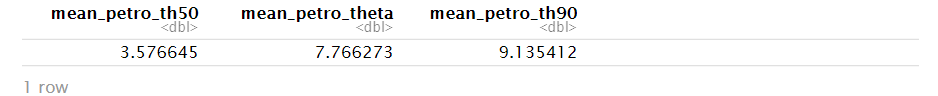
\includegraphics[width=0.8\textwidth]{Graphs/2.png}
	\caption{tibble containing the means of the variables petro\_th50, petro\_theta, and petro\_th90}
\end{figure*}


\begin{figure*}[h]
	\centering
	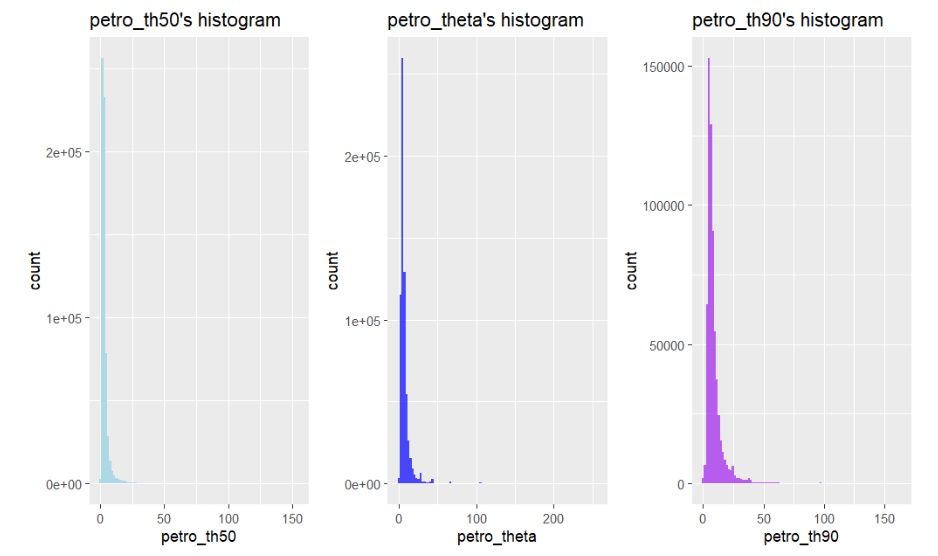
\includegraphics[width=0.7\textwidth]{Graphs/1.png}
	\caption{plot composition of three histograms (petro\_th50's histogram, petro\_theta's histogram and petro\_th90's histogram)}
\end{figure*}

\newpage 
\mbox{}
\newpage

\section{Updates in research question 2: Do the galaxies farthest to the Earth differ significantly from the closest ones in terms of their total luminosity?}

In addressing the research question number 2, the progress made so far is: We firstly cleaned the data to remove the NA values in both variables, `redshift' and `elpetro\_absmag\_r', which are used in the investigation of the question. Further, we measured the mean total luminosities of two samples of the galaxies that are situated closest to and furthest from the planet Earth. We illustrated the comparison of these two values using a bar graph.

\begin{figure*}[h]
	\centering
	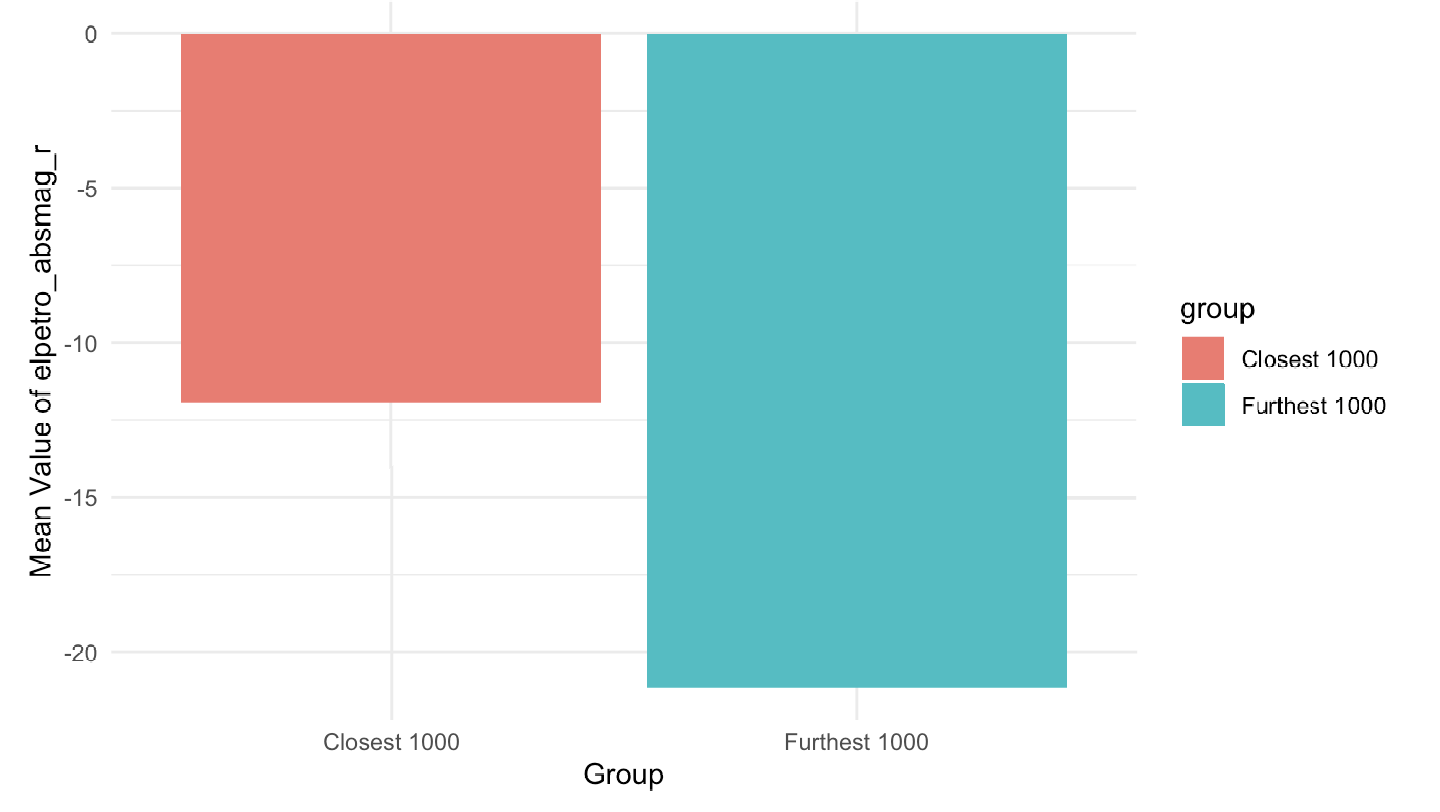
\includegraphics[width=0.8\textwidth]{Graphs/3.png}
	\caption{Comparison of Mean Values}
\end{figure*}

By doing so, we acquired the difference between actual measured values of total luminosities which we will use in the hypothesis test of the project. Subtracting one of these values from another, we will try to investigate the possibility of these two means being equal to or more extreme than this value under the null hypothesis, i.e. if there were no difference between the mean elpetro\_absmag\_r values of these two samples. The method that we used to find out these values was firstly arranging the data set in an increasing and then decreasing order of `redshift'. Next, we chose the top 1000 rows of both data frames and combined them in one single dataset. 

We also studied whether the difference in the means of these two samples is just a result of coincidence or there is an actual negative trend between the `elpetro\_absmag\_r' values and `redshift' values. In other words, we investigated if it is a common trend for the total luminosity to decrease as the galaxies get further from the Earth. To do so, we grouped each 1000 rows of the data frame where `redshift' is in an increasing order. Next, we illustrated the line graph of the mean `elpetro\_absmag\_r' values corresponding to each 1000-row group. 

\begin{figure*}[h]
	\centering
	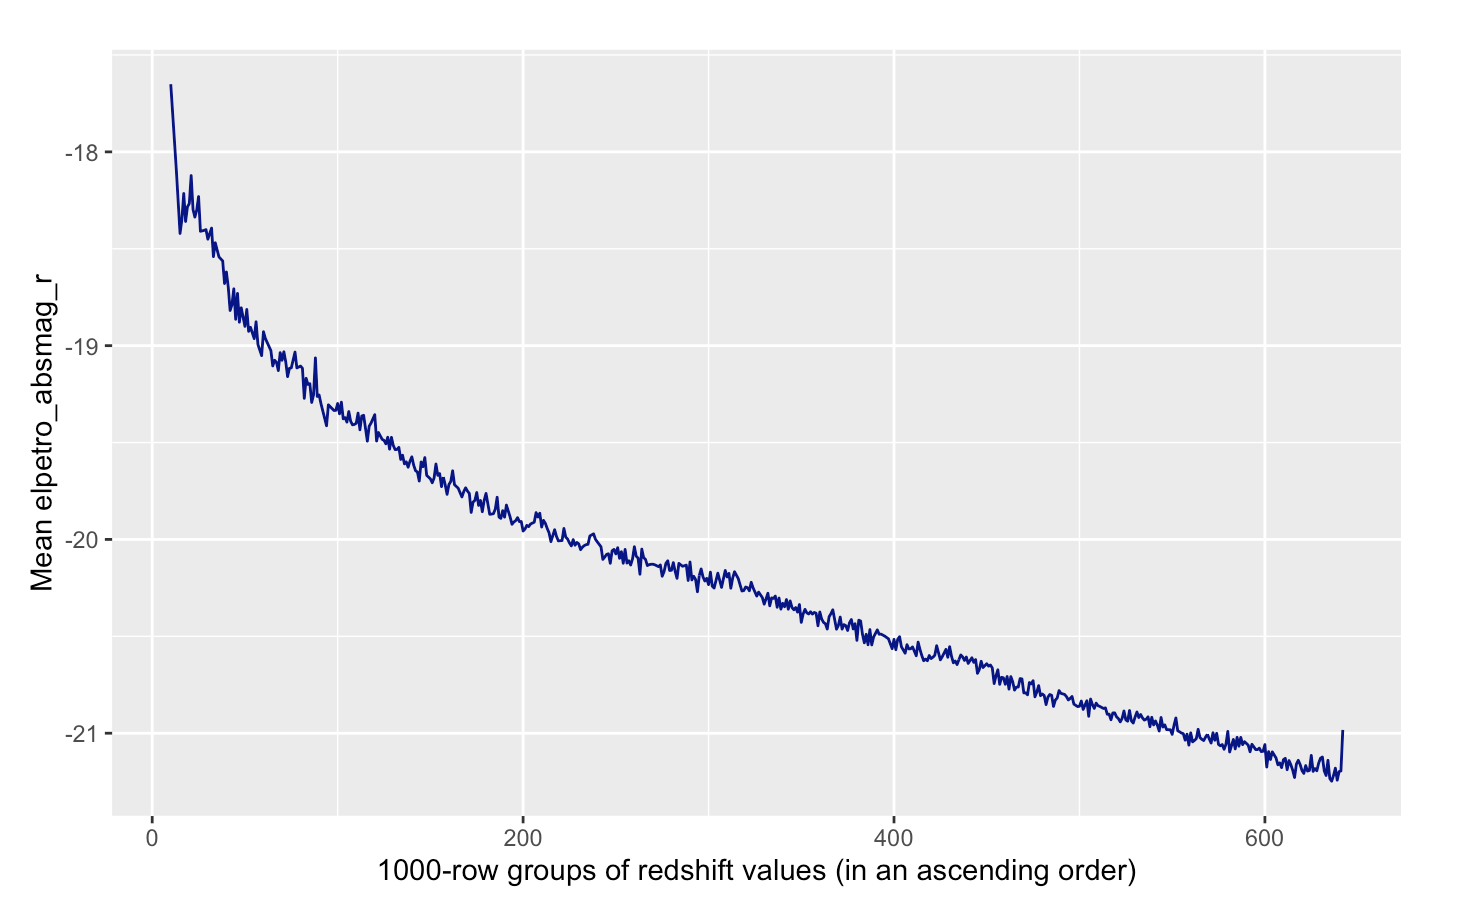
\includegraphics[width=0.8\textwidth]{Graphs/4.png}
\end{figure*}

In the second plot, x-axis corresponds to each group of 1000 galaxies that are ordered as per their red-shift values (from least to most) and y-axis is the mean `elpetro\_absmag\_r' of each group. 

One problem that we encountered while plotting this result was the outliers / unusual y values: The extreme `elpetro\_absmag\_r' means were distorting the shape of the graph, disfiguring the general trend and making it harder for the reader to follow the line. To tackle it, we removed the mean values that lay outside of the interquartile range (those higher than 75th percentile and lower than 25th percentile). After doing so, we got a more good-looking plot demonstrating an obvious downward tendency between the variables, and confirming our predictions.

\newpage

\section{Updates in research question 3:  How well can a unary linear regression model predict the galaxy's apparent brightness from redshift?}

\subsection{Updates in research question 3}
After carefully dived into the research, we didn't make any modification on research question for research question 3 as it keeps originally: How well can a unary linear regression model predict the galaxy's apparent brightness from redshift?

\subsection{Updates in data}
 The data we used in Research Question 3 comes from `Galaxy Zoo Tabular Data Contents'
 \begin{enumerate}
 	\item  Firstly, we loaded two different libraries: `tidyverse' and `arrow';
 	\item Secondly, we find the file by function (`arrow' library) and then use `read\_parquet' to read the second parquet (`nsa\_v1\_0\_1\_key\_cols.parquet'), and store it in `df2';
 	\item Thirdly we glimpse of this data by using the `glimpse' function (`tidyverse' library) to see the variable we will use.;
 	\item Finaly we use `filter' function to remove NA data from `df2'. We are good to graph.
 \end{enumerate}
 
\subsection{Updates in visualization}
\begin{figure*}[h]
	\centering
	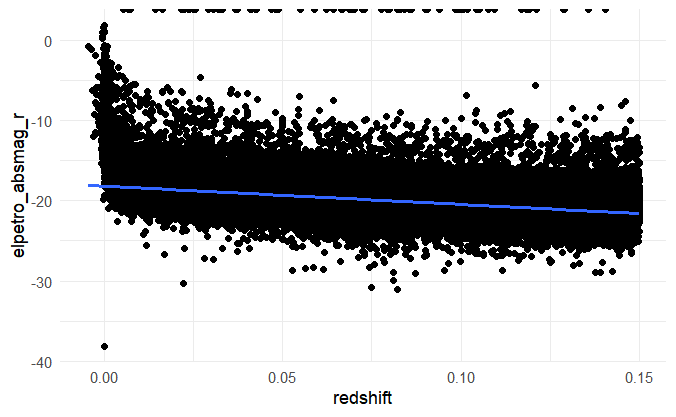
\includegraphics{Graphs/5.png}
	\caption{The Fitted Line Plot}
\end{figure*}

\subsection{Updates in method}
\begin{enumerate}
	\item We use `ggplot + geom\_point() + geom\_smooth + theme\_minimal()' function to create a linear regression plot. `redshift' is the x-axis, `elpetro\_absmag\_r' is the y-axis.
	\item After doing that, we use mod <- `lm' to create a `mod' the analysis the relationship between `redshif' and `elpetro\_absmag\_r', after that, we apply `summary\$coefficients' to find the B1, B0 and p-value. The B0 is the brightness when redshift equal to zero. B1 is the average change in brightness for 1 unit change in redshift.
	\item From here, we can do hypothesis test. $H_0$ will be There is a linear relationship between brightness and redshift. $H_1$ will be There is not a linear relationship between brightness and redshift. The p-value we got form summary will tell us whether to reject $H_0$.
\end{enumerate}



\newpage

\section{Potential Challenges}
Overall, some challenges exist during the process. Although there are three main aspects, the impact on our timeline is still manageable.  
\begin{enumerate}
	\item Time Constraints: This could include not having enough time to collect the necessary data, complete the analysis, or write up the report. These weeks, we are frequently having term tests, presentations and big assignments, therefore, time constraints definitely exists when we were writing the progress report. To deal with this, after finishing the exams, presentations and assignments, we prioritized tasks and focus on the most critical components of the project. This impacts the proposed timeline since we need to push back deadline we wrote in the proposal a bit. We made the main part finished 4 days later than we scheduled.
	\item Statistical analysis difficulties: Statistics can be a challenging subject, and we encountered difficulties with the statistical analysis when dealing with the dataset. The dataset we used in the capstone project is the most complex dataset we've seen in my entire live. his could include choosing the appropriate statistical tests or dealing with complex data structures. To deal with this, we need to seek assistance from our TA. This impacts the proposed timeline as well since we need to modify our project after receiving the suggestions. And should be one of the reasons why we finished the main part several days later.
	\item Technology issues: Technology issues is also a challenge in our capstone project. This could include difficulties with software or hardware, such as data analysis software, data storage or server issues, or compatibility issues with different systems. When analyzing data for research question 3, our PC overloaded and all of our logged data for research question 3 was lost. So we have to do it again, which should also be one of the reasons why we finished the main part several days later. 
	\item Communication challenges: Finally, communication challenges arise in statistics projects. Our capstone project group consists of colleagues from different countries. This could include difficulty communicating when discussing our ideas. To deal with this, we prepared and practiced effective communication strategies, such as using clear and concise language, visual aids, or examples before we had any discussion meetings. This could impact the proposed timeline since we need to spend additional time communicating with our teammates. 
\end{enumerate}

\newpage
\section{Contribution}
\begin{enumerate}
	\item Nicolas Dias Martins: Responsible for research question 1, who firstly share with other group members about their research questions as well as the dataset, methods, and visualizations they will use in research question 1. He also finished the main part (coding, analysis) of their own research questions. Besides writing the updates in research question 1 for project progress report, he also help with all the problems that our group faced during the process
	\item Riyad Valiyev: Responsible for research question 2, who also firstly share with other group members about their research questions as well as the dataset, methods, and visualizations they will use in research question 2. He finished the main part (coding, analysis) of their own research questions. Besides writing the updates in research question 2 for project progress report, he also help with all the problems that our group faced during the process
	\item Shujun Yang: Responsible for research question 3, who also firstly share with other group members about their research questions as well as the dataset, methods, and visualizations they will use in research question 3 with Xuanqi Wei. They shared their experiences and tell the difference between expectation and reality. Besides writing the updates in research question 3 for project progress report, she also help with all the problems that our group faced during the process.
	\item Xuanqi Wei: Responsible for research question 3, who also firstly share with other group members about their research questions as well as the dataset, methods, and visualizations they will use in research question 3 with Shujun Yang. They shared their experiences and tell the difference between expectation and reality. Besides integrate all the part for project progress report and writing the Potential Challenges and Contribution parts for project progress report, he also help with all the problems that our group faced during the process.
\end{enumerate}

We will make a table to visualize the contribution to make sure it's relatively equal.

\begin{table}[h]
\centering
\begin{tabular}{|c|c|c|c|c|c|} \hline
Names & Update RQ1 & Update RQ2 & Update RQ3 & Write PR & Integrate PR \\
\hline
	Nicolas Dias Martins & \checkmark & \ding{55} & \ding{55} & RQ1 & \ding{55} \\
\hline
	Riyad Valiyev & \ding{55} & \checkmark & \ding{55} & RQ2 & \ding{55} \\
\hline
	Shujun Yang & \ding{55} & \ding{55} & \checkmark & RQ3 & \ding{55} \\
\hline
	Xuanqi Wei & \ding{55} & \ding{55} & \checkmark & PC. and Con. & \checkmark \\ \hline
	
\end{tabular}
\end{table}

\noindent It is a pleasure to sincerely acknowledge our indebtedness to our TA, whom we warmly thank for his observation and suggestions, which materially improved the data processing process. 

\end{document}